\textit{Here we cover the RQ2, highlighting the challenge where although we have witnessed the growing adoption of Linked Open Data principles for publishing data on the Web, connecting data to third parties remains a difficult and time-consuming task. One question that often arises during the publication process is: ``Is there any data set available on the Web we can connect with?". This simple question unfolds a set of others that hinders data publishers to connect to other data sources. For instance, if there are related data sets, where are they? How many? Do they share concepts and properties? How similar are they? Is there any duplicated data set?
To answer these questions, this chapter introduces: (i) a new class of data repositories; (ii) a novel method to store and detect data set similarities (duplicated data set and data set chunks); (iii) an index to store data set relatedness; and, (iv) a search engine to find related data sets.
To create the index, we harvested more than 668k data sets from LOD Stats and LOD Laundromat, along with 559 active SPARQL endpoints corresponding to 221.7 billion triples or 5 terabytes of data. 
Our evaluation on state-of-the-art real-data shows that more than 90\% of data sets in the LOD Laundromat do not use the \textit{owl:equivalentProperty}, \textit{owl:equivalentClass} nor any other way to relate to one another data, which reaffirms ahd emphasize the importance of our work.}

\subsection{The ReLOD approach}
People will always describe knowledge in different ways, due to the individuality of the being, different points of view, time and space, in which we assume as a natural phenomenon and standard. Aware of the state of the art from Ontology/Schema/Instance Matching from Linked Data from venues such as \ac{VLDB}\footnote{Link to the official web site: \url{https://www.vldb.org/}}, \ac{OEAI}\footnote{Link to the official web site: \url{http://oaei.ontologymatching.org/}}, \ac{ISWC}\footnote{Link to the official web site: \url{https://iswc2019.semanticweb.org/}}, \ac{ESWC}\footnote{Link to the official web site: \url{https://2019.eswc-conferences.org/}}, among others, we observe that the \ac{LOD} datasets are following this standard.

We notice that there are several similar data sets. Yet, there is no place that stores or provides such kind of information about how similar the data sets are and which attributes the data sets share. This work aims to build an index to store the relation among the data sets to have a place to see how similar the data sets are. We provide a method to index the relations among LOD data sets\footnote{Data sets from LODStats, LODLaundromat, and endpoints} based on the properties and classes that they share.

As a motivation of our work, we describe two distinct scenarios where the proposed index may be useful:

\textbf{Scenario 1}: Given the SPARQL query at \cref{lst:scenario1}, where the user wants to know if a given data set contains three properties, in which the user already know the query performs well at the SPARQL endpoint from CKAN\footnote{  CKAN SPARQL endpoint~\url{https://linked.opendata.cz/sparql}}:

\begin{lstlisting}[language=SPARQL, label={lst:scenario1}, caption=Scenario 1.]
SELECT * WHERE { ?s ?p ?o.
FILTER(?s=<http://purl.org/dc/terms/date> || 
?s=<http://crime.rkbexplorer.com/id/location> || 
?s=<http://purl.org/dc/terms/subject>
)}
\end{lstlisting}
The following questions are raised:
\begin{itemize}
    \item How to know which data sets are able to execute the query?
    \item Which of the data sets contains the most valuable results?
    \item Could the results from different data sets complement each other?
\end{itemize}

In this case an approach is needed to enable the user to know more datasets to extract the required information. An index of dataset relations/similarities could be used to know that the query can also be executed with results at \url{https://eu.dbpedia.org/sparql} but not at \url{http://dbpedia.org/sparql}, and we can execute at least in other five\footnote{Datasets available here: \url{https://tinyurl.com/5dataset}} data sets to complement the results.

\textbf{Scenario 2}: The user need information about cities from all datasets in your repository, more specifically datasets that are compatible with the class \url{http://dbpedia.org/ontology/City}. Using our previous approach WIMU\cite{valdestilhas2018my}, this URI was found in 11 datasets\footnote{Datasets available here: \url{https://tinyurl.com/wimuDbpediaCity}}, but how many URIs in other datasets that also represents a city that were not listed, for instance a city at WikiData\footnote{Link to the official web site:  \url{https://www.wikidata.org/}} is represented by  \url{https://www.wikidata.org/wiki/Property:P131}.
We consider here that to execute such task manually on more than 600,000 datasets is not feasible. Thus, having an index of dataset relation will help in this case.

The contributions of this chapter are:
\begin{itemize}
    \item A method to create an incremental index of similarity among LOD datasets. Thus, to the best of our knowledge, ReLOD is the first dataset relation index over a net total of 221.7 billion triples.
    \item A creation of a mechanism to search this index by Dataset URI, property, class or SPARQL query. For the first time, to the best of our knowledge, we make a relation index able to query by dataset URI, property, class or SPARQL query.
    \item A method to identify duplicated datasets and chunks.
\end{itemize}

The rest of the chapter is organized as follows:
First we present our approach in the Section \ref{sec:approach} then the Section \ref{ev:relod} shows the evaluation results and discussion.

\subsection{The approach}
\label{sec:approach}
Our observations guide us to a method to create an index of LOD datasets, in which involves a compilation of many other works, starting collecting data from more than 650,000 LOD datasets from LODStats, LODLaundromat and more than 500 endpoints\footnote{The list of endpoints is available here: \url{https://github.com/firmao/wimuT/blob/master/Endpoints_numtriples_lodcloud.csv}}. 

%Among the steps we should hightlight the creation of a \textbf{Dataset catolog}, section\ref{sec:lodCatalog}, providing an efficient way to obtain all properties and classes from each dataset and an \textbf{approach to identify the namespace} of each dataset, described at section\ref{sec:namespace}, avoiding the necessity to open each dataset in order to know what more the domain of the dataset.

\subsubsection{The index creation}
\label{sec:indexCreation}

Given a set of Datasets $\mathbf{D}\{d_1,...,d_n\}$, assuming $d_n$ represents a RDF dataset\footnote{RDF datasets: \url{https://www.w3.org/TR/rdf11-datasets/}}, in which each $d$ contains a set of properties and classes represented by $\mathcal{P}$. The next step consists in creating a set $\mathbf{E}$ containing the identified duplicated datasets. Thus, we can exclude from $\mathbf{D}$ all datasets contained in $\mathbf{E}$.

The goal of algorithm \ref{alg:indexCreation}\footnote{Implementation in Java \url{https://tinyurl.com/y597qrah}} is to create an index to store the relations among datasets by comparing the occurrences of classes and properties of each dataset, by String similarity and Instance Matching. The \textbf{Input} is a set of Datasets and the \textbf{Output} is the index of dataset relations.

figure \ref{fig:create} shows a workflow about how the index is created and the algorithm \ref{alg:indexCreation} describe with more details the process of creation of the dataset relation index.

\begin{figure}[htb] 
	\centering
	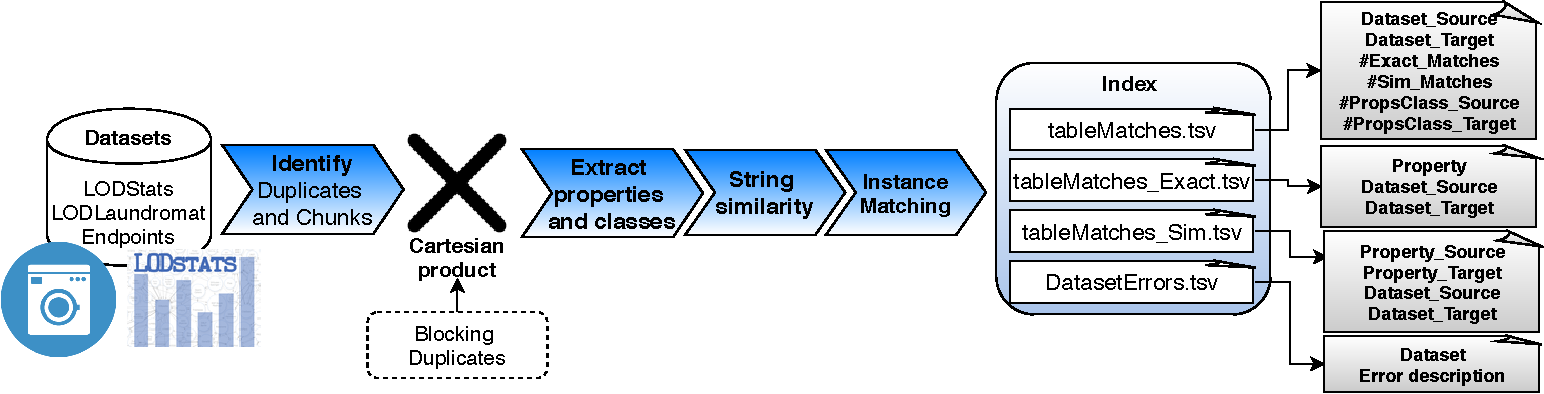
\includegraphics[width=\linewidth]{img/createIndex.pdf}
	\caption{Creating the index.}
	\label{fig:create}
\end{figure}

\begin{figure}[htb] 
	\centering
	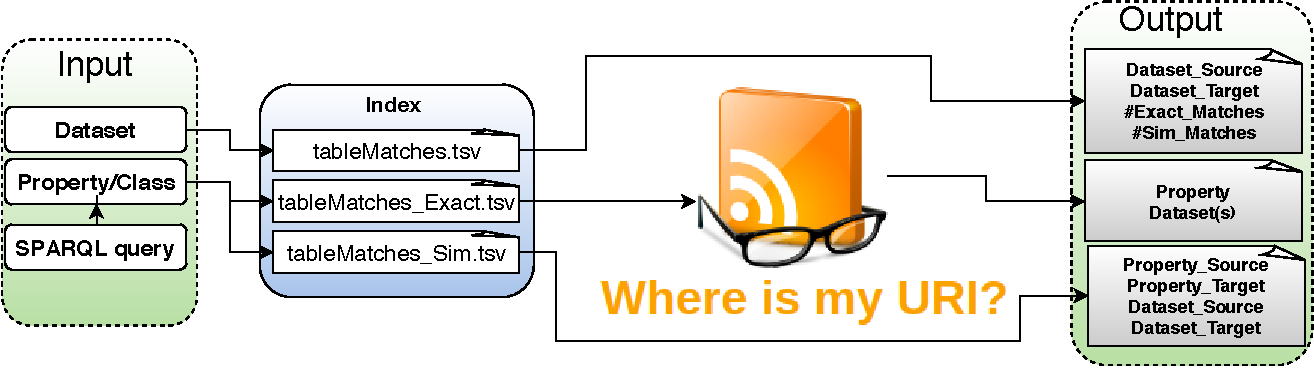
\includegraphics[width=\linewidth]{img/queryIndex.pdf}
	\caption{Querying the index.}
	\label{fig:queryIndex}
\end{figure}

\begin{algorithm} [htb] 
	\caption{Creation of the LOD dataset relation index}
	\label{alg:indexCreation}
    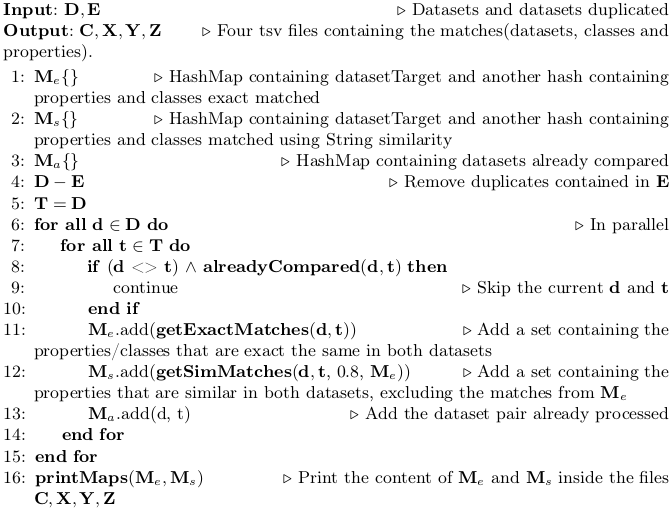
\includegraphics[width=\linewidth]{sections/img/algReLOD.png}
\end{algorithm}

% \begin{algorithm} [htb] 
% \caption{Creation of the LOD dataset relation index}
% \label{alg:indexCreation}
% \begin{lstlisting}[language=C, basicstyle=\large]
% Input:D,E //Datasets and datasets duplicated
% Output:C,X,Y,Z //Four tsv files containing the matches(datasets,classes and properties).
% Me{} //HashMap containing dataset Target and another hash containing properties and classes exact matched 
% Ms{} //HashMap containing dataset Target and another hash containing properties and classes matched using String similarity
% Ma{} //HashMap containing datasets already compared
% D-E //Remove duplicates contained in E
% T=D 
% for all d in D do //In parallel
%     for all t in T do
%         if (d<>t) and alreadyCompared(d,t) then
%             continue //Skip the current d and t
%         end if
%         Me.add(getExactMatches(d,t)) //Add a set containing the properties/classes that are exact the same in both datasets 
%         Ms.add(getSimMatches(d,t,0.8,Me)) //Add a set containing the properties that are similar in both datasets, excluding the matches from Me
%         Ma.add(d, t) //Add the dataset pair already processed 
%     end for
% end for
% printMaps(Me,Ms) //Print the content of Me and Ms inside the files C,X,Y,Z.
% \end{lstlisting}
% \end{algorithm}

The function \textbf{getExactMatches}($\mathbf{d},\mathbf{t}$)) compares all properties and classes from each dataset $\mathbf{d}$ and $\mathbf{t}$ and return a set of properties and classes that are exact the same, keeping the provenance of the dataset.

The function \textbf{getSimMatches}($\mathbf{d},\mathbf{t}$, 0.8, $\mathbf{M}_e$) compares all properties and classes from each dataset $\mathbf{d}$ and $\mathbf{t}$ using Jaccard and MFKC\cite{valdestilhas2017high} String Similarity function with a threshold of 0.8, excluding the exact matches identified previously by the function \textbf{getExactMatches} returning a set of properties and classes that has the similary greater than the threshold 0.8, keeping the provenance of the dataset, the figure \ref{fig:simMatch} shows our string similarity process.
\begin{figure}[htb] 
	\centering
	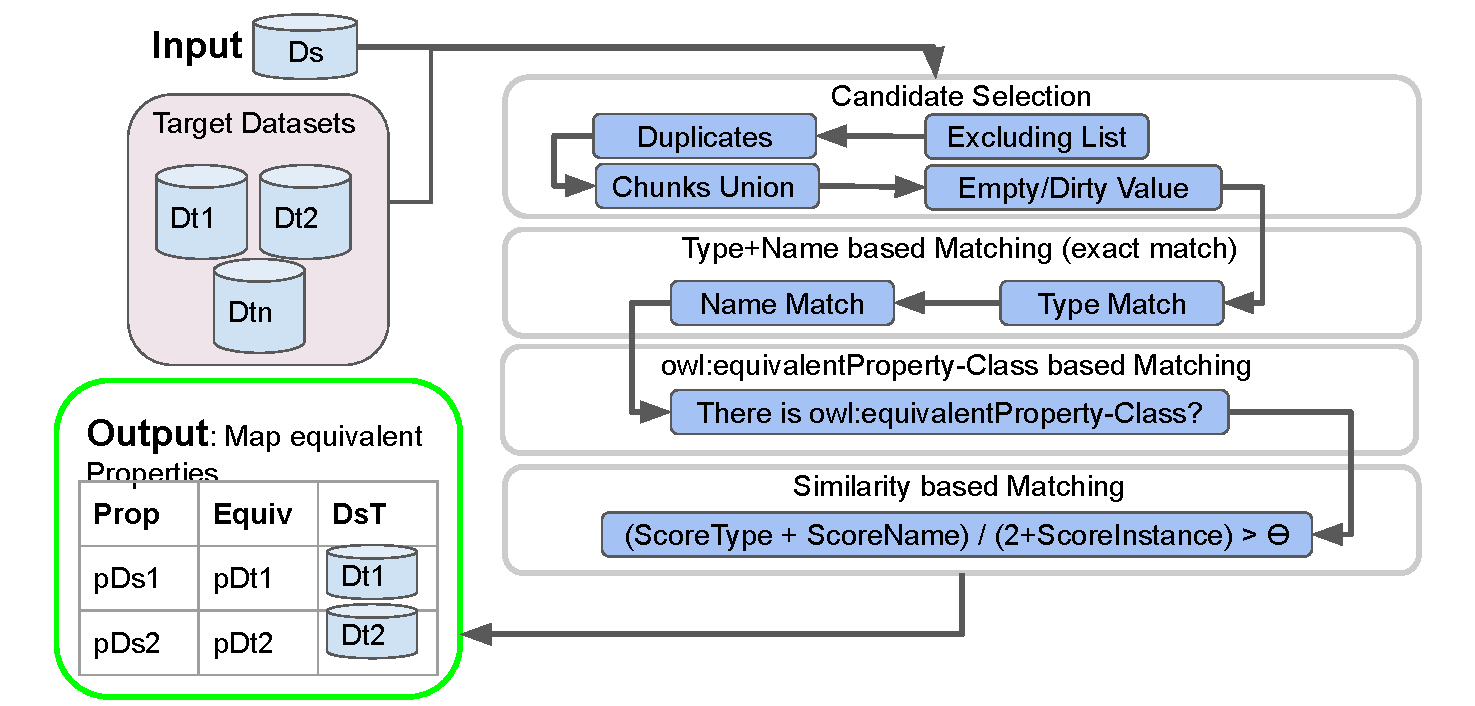
\includegraphics[width=\linewidth]{img/stringSim.pdf}
	\caption{String similarity process.}
	\label{fig:simMatch}
\end{figure}

The function \textbf{printMaps}($\mathbf{M}_e, \mathbf{M}_s$) print the content from the matching functions into the files according the structure described in section \ref{sec:FileStructure}.

\subsubsection{Identifying duplicated and chunk datasets}
\label{sec:duplicates}
With the current hardware available (HD 1Tb, Memory 16GB, processor intel core i7).
To compare all LOD datasets, in this case more than 600 thousand datasets, implies in more than 360 billion of comparisons($n*n$), assuming that each comparison takes in average 1 millisecond, the whole operation will take more than 10 years.

Thus, we decided to have a blocking method to avoid unnecessary comparisons. To this aim, we create a way to detect duplicated and chunk-dump-files datasets, described on \cref{alg:dupchunk}. 
Our blocking method avoid datasets with less than 1 triple, duplicates, less than 5 properties, less than 5 classes.

The function \textbf{eliminateDuplicates()}, identify and eliminate duplicated HDT files by comparing the property occurrences of each dataset and the header metadata.

We formalize the problem of Clustering datasets identifying duplicates and chunks as follows:

We consider a set of $\mathbf{K}$ data sources $\mathbf{S_1}, . . . , \mathbf{S_k}$ containing property occurrences $\mathbf{O_1}, . . . , \mathbf{O_m}$. Each of property $\mathbf{P}$ is referenced by an \texttt{URI}, e.g., dbo:City\footnote{dbo:City states for the URI \url{http://dbpedia.org/ontology/City}}. Each $\mathbf{S}$ contains a header $\mathbf{H}$, with meta-data about the data in $\mathbf{S}$, such that $\mathbf{H} \subset \mathbf{S}$.

The goal is to create clusters of datasets $\mathbf{C}$ in two groups of elements from $\mathbf{K}$, in which are duplicates $\mathbf{D}$ and chunks $\mathbf{E}$, such that $\mathbf{D} \subset \mathbf{K} : \mathbf{E} \subset \mathbf{K} : \mathbf{K} \subset \mathbf{C}$.

We assume that all datasets are not empty and are RDF compatible with the HDT format.

Firstly we create a dense matrix of property occurrence and dataset. Then it was observed a standard in the dense matrix, that for some datasets the occurrence of the properties was exactly the same. Then, we identify that we can put together those datasets to observe more characteristics.
In this second phase, we have a sub-collection of our initial collection of datasets and looking into the header metadata of those files we observe that for some files the meta-data is different. Then we have another sub-collection of files with different headers, and manually reading file by file we realize that they are chunks, in other words, part of a bigger dataset. 

Thus we have two phases for clustering dataset (1) Put together datasets that present the same occurrence of properties. (2) Read the header metadata and separate files with a different header. The files with different header are chunks and the rest are duplicates\footnote{More details, please see the implementation and the documentation on \url{https://github.com/firmao/wimuT} and the specific implementation java class for this task: \url{https://github.com/firmao/wimuT/blob/master/src/org/wimu/datasetselection/parallelv1/ClusterKmeans.java}}.

% \begin{figure}[htb] 
% 	\centering
% 	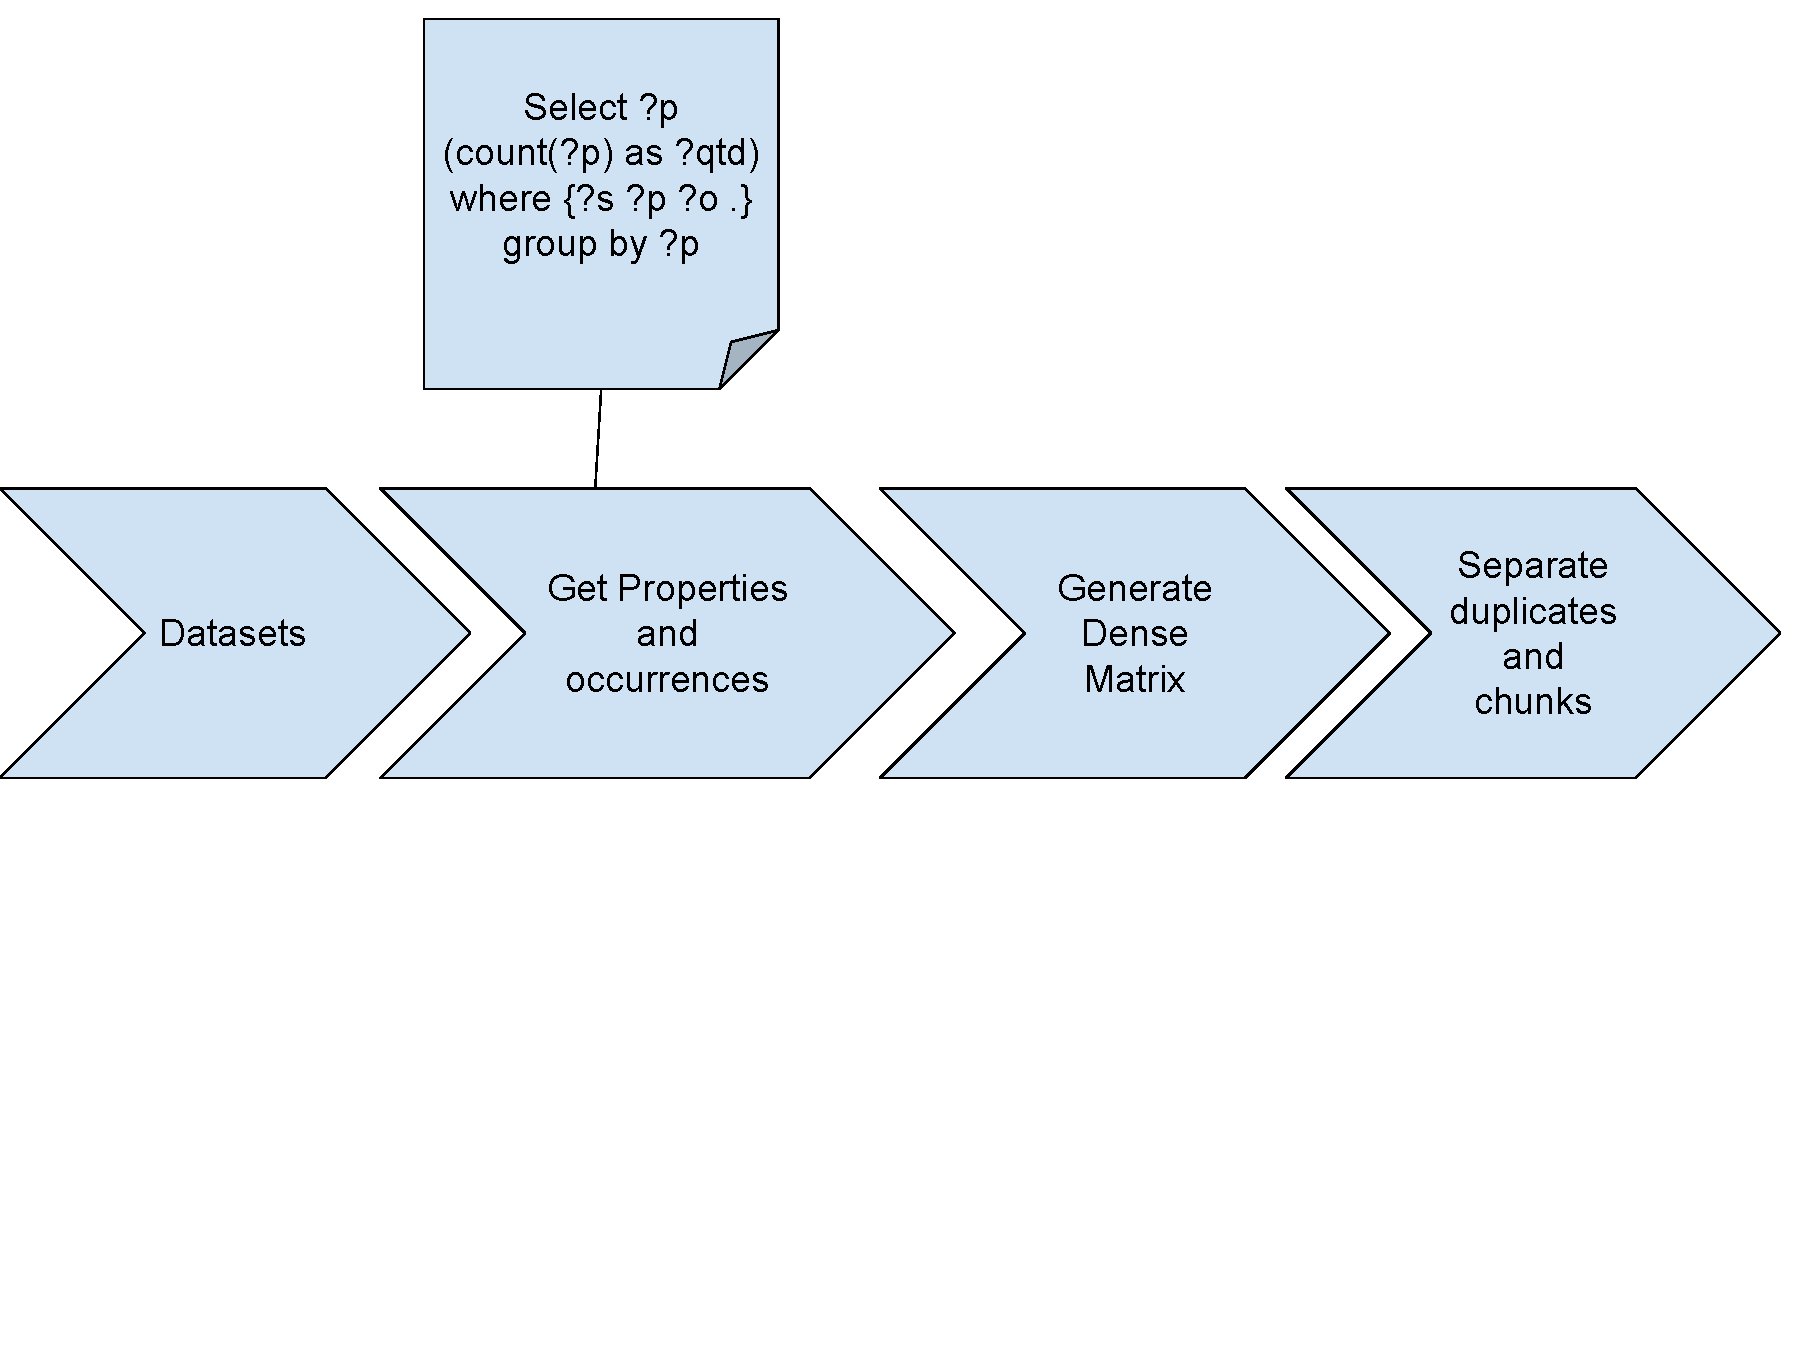
\includegraphics[width=\linewidth]{img/duplicates.pdf}
% 	\caption{Identifying duplicates and chunks.}
% 	\label{fig:duplicates}
% \end{figure}

\begin{algorithm} [htb] 
	\caption{Identifying duplicates and chunk}
	\label{alg:dupchunk}
    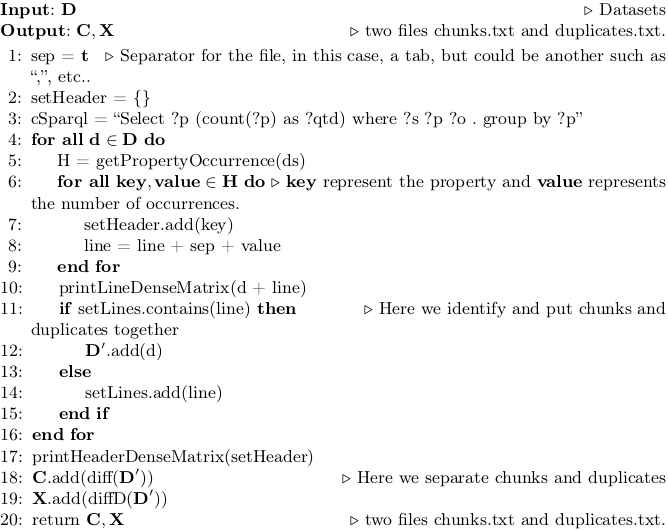
\includegraphics[width=\linewidth]{sections/img/algDupChunk.png}
\end{algorithm}   

% \begin{algorithm}
% 	\caption{Identifying duplicates and chunk}
% 	\label{alg:dupchunk}
% \begin{lstlisting}[language=C, basicstyle=\large]
% Input:D //Datasets
% Output:C,X //Two files chunks.txt and duplicates.txt
% sep = t //Separator for the file, in this case, a tab, but could be another such as ',', etc.
% setHeader = {} 
% cSparql = ''Select ?p (count(?p) as?qtd) where ?s ?p ?o . group by ?p''
% for all d in D do
%     H = getPropertyOccurrence(ds)
%     for all key,value in H do //key represent the property and value represents the number of occurrences.
%         setHeader.add(key)
%         line = line + sep + value
%     end for
%     printLineDenseMatrix(d + line)
%     if setLines.contains(line) then //Here we identify and put chunks and duplicates together
%         D'.add(d)
%     else
%         setLines.add(line)
%     end if
% end for
% printHeaderDenseMatrix(setHeader)
% C.add(diff(D')) //Here we separate chunks and duplicates
% X.add(diffD(D'))
% return C,X //Two files chunks.txt and duplicates.txt.
% \end{lstlisting}
% \end{algorithm}

The function \textbf{getPropertyOccurrence}(ds) returns a hash map containing the property and the number of occurrences of each property from a given dataset with the SPARQL query at \cref{lst:propOccur1} 

\begin{lstlisting}[language=SPARQL, label={lst:propOccur1}, caption=Property occurrence query.]
Select ?p (count(?p) as ?qtd) where {?s ?p ?o .} group by ?p
\end{lstlisting}
The function \textbf{printLineDenseMatrix}(line) print a line in a file and the function \textbf{printHeaderDenseMatrix}(setHeader) print the first line of the dense matrix file containing the header of the matrix, in which refers to the identification of the properties.
The function \textbf{diff}($\mathbf{D’}$ ) separates the chunks from duplicates, for this task we look into the header of the files, in this case, only HDT files, where duplicates present exactly the same header metadata information and chunks are different respect to the header.

\textbf{Theorem 1}: Let $\mathbf{P}$ be a collection of property occurrences of datasets $\mathbf{D}$, such that each $\mathbf{D}$ has one $\mathbf{P}$, in which $\mathbf{D’}$ represents the cluster candidates, in which are the datasets identified as chunks and duplicates together, and the function \textbf{diff()} return the dump-files that are not duplicated. Thus, the output of Algorithm 1 when applied to $\mathbf{D}$, the following hold:

$|\textbf{diff}(\mathbf{D’})| = 0$

All elements from $\mathbf{D’}$ are duplicated datasets.


To identify the chunks:

$|\textbf{diff}(\mathbf{D’})| > 0$


The result from $\textbf{diff}(\mathbf{D’})$ are the dump-files identified as chunks.

% \subsection{The LOD catalog - Class property index}
% \label{sec:lodCatalog}
% \todo[inline]{Claus, when you are ready let's put your work here and some experiments/evaluation later. I also need to adapt my code to yours.}

% \subsection{Relating the name spaces with dataset names}
% \label{sec:namespace}
% The datasets from LODLaundromat\cite{} are identified with a MD5 code\footnote{ref MD5}, e.g \texttt{009e80050fa7f4279596956477157ec2.hdt}\footnote{\url{http://139.18.13.76:8082/dirHDTLaundromat/decompressed/00/009e80050fa7f4279596956477157ec2/009e80050fa7f4279596956477157ec2.hdt}} represent a dataset from the domain \texttt{knoesis.wright.edu} in which is a dataset about \textit{The Ohio Center of Excellence in Knowledge-enabled Computing (Kno.e.sis)}.

% We developed a method to convert the MD5 code from the HDT to URLs with more informative name spaces, instead of the MDA code we have the name space of the dataset giving us more information about the dataset avoiding the need to open the HDT file to obtain this information.

% The Algorithm \cref{alg:Edgard} describes how we create this complementary index.

% \todo[inline]{Edgard, please describe the algorithm when is better for you. And some evaluation.}

% \begin{table}[]
% \begin{tabular}{@{}lcccc@{}}
% \toprule
% \textbf{Process}           & \multicolumn{1}{l}{\textbf{Runtime}} \\ \midrule
%  Complete Namespace extraction & ?             \\              
%  Dominant Namespace extraction & ?             \\              Index creation    & ?               \\
%  \bottomrule
% \end{tabular}
% \end{table}

\subsubsection{The file structure}
\label{sec:FileStructure}

Now we describe the file structure that we created to use our index, which consists of 3 TSV\footnote{Tab Separated Value(TSV)} files.
\begin{itemize}
    \item $\textbf{tableMatches\_Exact.tsv}$: Contains the exact match of the properties, with the following fields: 
    \begin{itemize}
        \item \textbf{Property}: containing the property URI itself.
        \item \textbf{Source}: Contains the dataset source where the property was found.
        \item \textbf{Target}: Contains de dataset matched containing the property.
    \end{itemize}
    \item $\textbf{tableMatches\_Sim.tsv}$: Represents the similarity of properties from datasets Source and Target, with the following fields:
    \begin{itemize}
        \item \textbf{PropertyS}: The property from the dataset Source.
        \item \textbf{PropertyT}: The property from the dataset Target.
        \item \textbf{Source}: The dataset Source.
        \item \textbf{Target}: The dataset Target.
    \end{itemize}
    \item \textbf{tableMatches.tsv}: Represents the datasets Matched and his respectives number of properties exact matched and number of properties matched with String similarity, with the following fields:
    \begin{itemize}
        \item \textbf{Source}: The dataset source.
        \item \textbf{Target}: The dataset Target.
        \item $\textbf{\#ExactMatch}$: Number of properties with exact match.
        \item $\textbf{\#sim>0.9}$: Number of properties with similarity threshold greater than 0.9.
    \end{itemize}
\end{itemize}

\subsubsection{Querying the index}
%\todo[inline]{Describe how to query the index, how the web prototype do the task: \url{https://github.com/firmao/LODDatasetRelationsWeb}} 

The index provides the following information based on three types of input:
\begin{description}
    \item \textbf{Dataset}: The index will provide a list of datasets, number of exact matched\footnote{Exact Match where the URI is exact the same following the principle of uniqueness of the URI} properties and number of similar\footnote{Similarity match occurs when the similarity of the URI is greater than 0.9 if less we perform Instance matching.} properties.
    \item \textbf{Set of properties (URIs) separeted by comma}: 
    \begin{itemize}
        \item Json file containing the property and the list of datasets where this property were found by exact match.
        \item A table containing the matches by similarity with the following fields:
        \begin{description}
            \item \textbf{Property Source}: Representing the property found on the dataset source.
            \item \textbf{Property Target}: Representing the property found on the dataset target.
            \item \textbf{Dataset Source}: The name of the dataset source.
            \item \textbf{Dataset Target}: The name of the dataset target.
        \end{description}
    \end{itemize}
    \item \textbf{SPARQL query}: This type of input extracts the set of properties from the SPARQL query and performs the same operation as \textbf{Set of properties (URIs) separeted by comma}.
\end{description}

The index is also incremental, allowing to add more datasets to be processed once a month\footnote{Once a month due to the the time to generate that with our hardware takes at least 88 hours}.
The prototype is available online for proof of concept online\footnote{Link to the prototype: \url{http://w3id.org/relod/}} and the figure \ref{fig:queryIndex} shows a workflow about how the index is used.



% \todo[inline]{try with elasticsearch and see if is better or not.}
% \begin{verbatim}
% elasticsearch_loader <options> csv --delimiter '\t' filename.tsv

% https://www.reddit.com/r/elasticsearch/comments/at7huu/how_can_i_import_tsv_to_elasticsearch/
% \end{verbatim}

%The figure \ref{fig:datasetMatch},figure \ref{fig:exactMatch}, figure \ref{fig:similarMatch} show 3 examples of 3 different types of results to 3 different queries to the index.

% \begin{figure}[htb] 
% 	\centering
% 	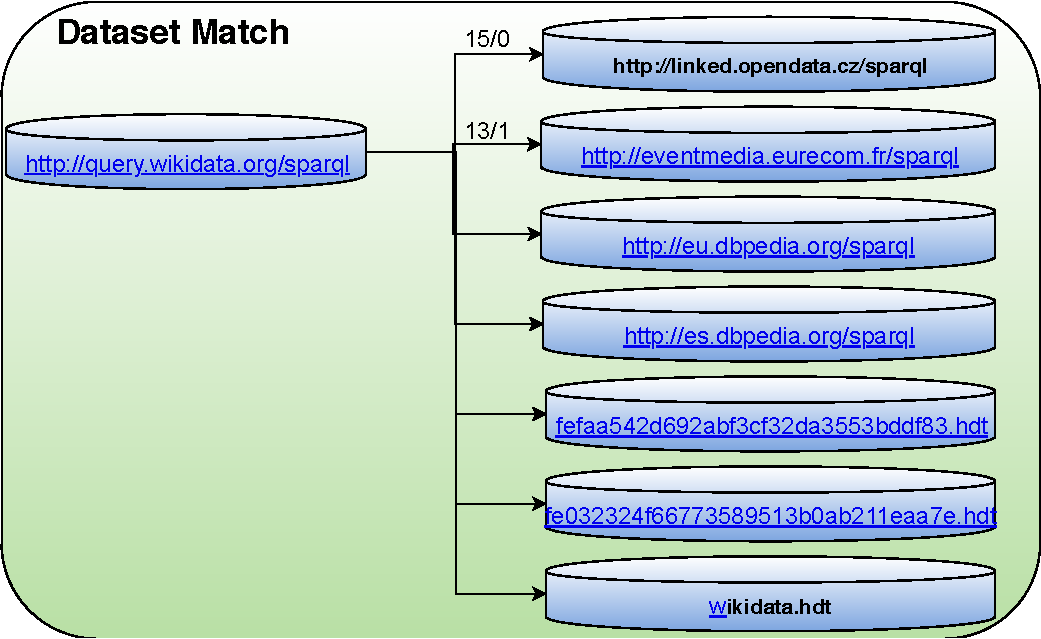
\includegraphics[width=\linewidth]{llncs/img/datasetMatch.pdf}
% 	\caption{Example of dataset match.}
% 	\label{fig:datasetMatch}
% \end{figure}

% \begin{figure}[htb] 
% 	\centering
% 	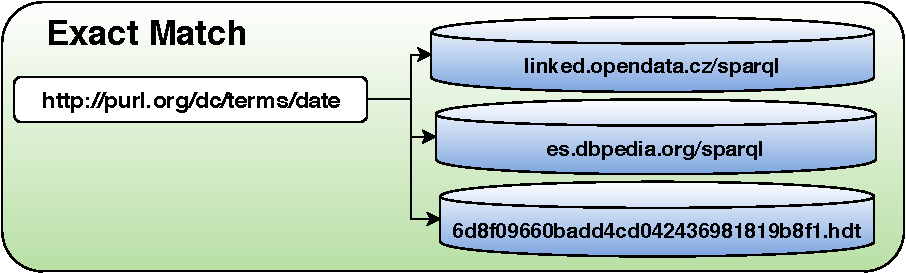
\includegraphics[width=\linewidth]{llncs/img/exactMatch.pdf}
% 	\caption{Example of exact match.}
% 	\label{fig:exactMatch}
% \end{figure}

% \begin{figure}[htb] 
% 	\centering
% 	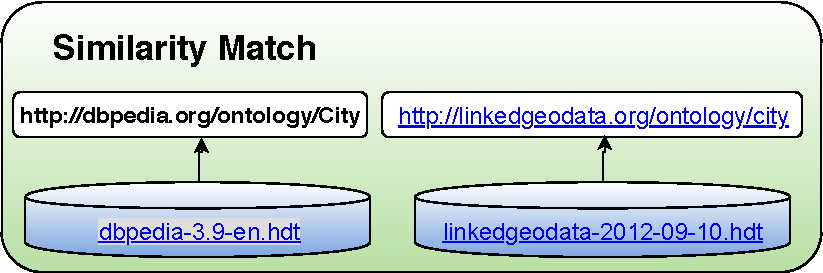
\includegraphics[width=\linewidth]{llncs/img/similarMatch.pdf}
% 	\caption{Example of similar match.}
% 	\label{fig:similarMatch}
% \end{figure}

% \begin{figure}[htb] 
% 	\centering
% 	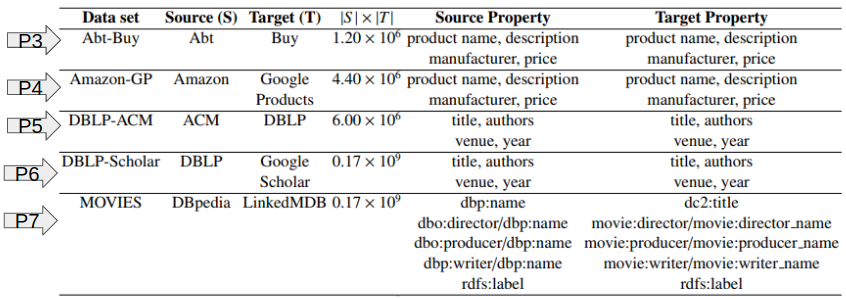
\includegraphics[width=\linewidth]{llncs/img/goldESWCKleanthi.png}
% 	\caption{Sample datasets from \cite{georgala2018dynamic} to evaluate our string similarity approach.}
% 	\label{fig:TableFmeasure}
% \end{figure}

\begin{table}[htb]
\centering
\caption{Sample datasets from \cite{georgala2018dynamic} to evaluate our string similarity approach.}
\label{tab:TableFmeasure}
\rotatebox{90}{
\resizebox{1.7\linewidth}{!}
{
\begin{tabular}{*{6}{c}} \hline
    \textbf{Data set}           & \textbf{Source (S)} & \textbf{Target (T)} & \textbf{$|S| \times |T|$} & \textbf{Source Property} & \textbf{Target Property}                           \\ \hline
    
    \textbf{(P3)}Abt-Buy    & Abt & Buy  & $1.20 \times 10^6$ & product name, description                       & product name, description                         \\
                                &&&& manufacturer, price               & manufacturer, price                       \\ \hline
    \textbf{(P4)}Amazon-GP  & Amazon & Google & $4.40 \times 10^6$ & product name, description                 & product name, description                         \\ 
                                && Products && manufacturer, price               & manufacturer, price                       \\ \hline
    \textbf{(P5)}DBLP-ACM  & ACM & DBLP& $6.00 \times 10^6$ & title, authors                    & title, authors                            \\
                                &&&& venue, year                       & venue, year                               \\ \hline
    \textbf{(P6)}DBLP-Scholar& DBLP & Google  & $ 0.17 \times 10^9$ & title, authors                    & title, authors                            \\
                                && Scholar && venue, year                       & venue, year                               \\ \hline
    \textbf{(P7)}MOVIES   & DBpedia & LinkedMDB & $0.17 \times 10^9$ & dbp:name                          & dc2:title     \\
                                &&&& dbo:director/dbp:name             & movie:director/movie:director\_name       \\
                                &&&& dbo:producer/dbp:name             & movie:producer/movie:producer\_name       \\
                                &&&& dbp:writer/dbp:name            & movie:writer/movie:writer\_name           \\
                                &&&& rdfs:label & rdfs:label           \\ 
                                \hline
\end{tabular}
}}
\end{table}


\subsection{Evaluation}
\label{ev:relod}
This evaluation aims to answer the following questions: (1) How to identify and quantify similar datasets for a given Dataset?\footnote{To know how many datasets are similar to each other.} (2) How many datasets are most likely to execute a given SPARQL query? (3) How the detection of duplicated and chunk datasets can help in the process of matching a large amount of datasets? (4) How ReLOD increase the number of datasets identified by wimuQ?

The information contained at table \ref{tab:simJaccard} and table \ref{tab:contained} are used to see how a sample of datasets are similar, we take 8 famous datasets from \textit{rdfhdt.org}\footnote{Link to the official web site: \url{http://www.rdfhdt.org/datasets/}} and 12 from \cite{10.1145/3308560.3317075}. To obtain the results from the table \ref{tab:simJaccard}. which is to see how similar are the datasets, we use the formula \cref{eq:jaccard} and to obtain the results from table \ref{tab:contained}, to see how much a dataset is contained inside each other we use the formula in the equation \ref{eq:contained}, where A and B represents datasets source and target. We have an alternative way to visualize this sample data as a graph\footnote{Link to visualize the relation graph: \url{https://w3id.org/relod/visual.html}}.

\begin{equation} \label{eq:jaccard}
    jaccard(A, B) = \frac{|A \bigcap B|}{ |A\bigcup B|}
\end{equation}

\begin{equation}\label{eq:contained}
    contained(A, B) = \frac{|A \bigcap B|}{|A|}
\end{equation}

\begin{table}[ht]
\centering
\resizebox{\textwidth}{!}{
\rotatebox{90}{
\begin{tabular}{|c|l|l|l|l|l|l|l|l|l|l|l|l|l|l|l|l|l|l|l|l|}
\hline
\textbf{\rotatebox{45}{Coeficient}} & \textbf{\rotatebox{90}{acadonto}} & \textbf{\rotatebox{90}{acm.rkbexplorer}} & \textbf{\rotatebox{90}{agrinepaldata}} & \textbf{\rotatebox{90}{aims}} & \textbf{\rotatebox{90}{alaska}} & \textbf{\rotatebox{90}{apertium}} & \textbf{\rotatebox{90}{arrayexpress}} & \textbf{\rotatebox{90}{athelia}} & \textbf{\rotatebox{90}{bfs.270a}} & \textbf{\rotatebox{90}{biblioteca-nacional}} & \textbf{\rotatebox{90}{brown}} & \textbf{\rotatebox{90}{dblp}} & \textbf{\rotatebox{90}{dbpedia}} & \textbf{\rotatebox{90}{geonames}} & \textbf{\rotatebox{90}{linkedgeodata}} & \textbf{\rotatebox{90}{swdf}} & \textbf{\rotatebox{90}{vivosearch}} & \textbf{\rotatebox{90}{wiktionary}} & \textbf{\rotatebox{90}{wordnet}} & \textbf{\rotatebox{90}{yago}} \\ \hline
\textbf{acadonto} & \cellcolor{green!100.0}1.0 & \cellcolor{green!2.0}0.02 & \cellcolor{green!11.0}0.11 & \cellcolor{green!5.0}0.05 & \cellcolor{green!0.0}0.00 & \cellcolor{green!3.0}0.03 & \cellcolor{green!2.0}0.02 & \cellcolor{green!6.0}0.06 & \cellcolor{green!1.0}0.01 & \cellcolor{green!2.0}0.02 & \cellcolor{green!2.0}0.02 & \cellcolor{green!2.0}0.02 & \cellcolor{green!0.0}0.00 & \cellcolor{green!2.0}0.02 & \cellcolor{green!0.0}0.00 & \cellcolor{green!1.0}0.01 & \cellcolor{green!1.0}0.01 & \cellcolor{green!2.0}0.02 & \cellcolor{green!1.0}0.01 & \cellcolor{green!2.0}0.02  \\ \hline
\textbf{acm.rkbexplorer} & \cellcolor{green!2.0}0.02 & \cellcolor{green!100.0}1.0 & \cellcolor{green!8.0}0.08 & \cellcolor{green!22.0}0.22 & \cellcolor{green!1.0}0.01 & \cellcolor{green!11.0}0.11 & \cellcolor{green!1.0}0.01 & \cellcolor{green!28.999999999999996}0.29 & \cellcolor{green!30.0}0.30 & \cellcolor{green!7.000000000000001}0.07 & \cellcolor{green!20.0}0.20 & \cellcolor{green!5.0}0.05 & \cellcolor{green!0.0}0.00 & \cellcolor{green!2.0}0.02 & \cellcolor{green!0.0}0.00 & \cellcolor{green!2.0}0.02 & \cellcolor{green!1.0}0.01 & \cellcolor{green!4.0}0.04 & \cellcolor{green!2.0}0.02 & \cellcolor{green!8.0}0.08  \\ \hline
\textbf{agrinepaldata} & \cellcolor{green!11.0}0.11 & \cellcolor{green!8.0}0.08 & \cellcolor{green!100.0}1.0 & \cellcolor{green!11.0}0.11 & \cellcolor{green!1.0}0.01 & \cellcolor{green!16.0}0.16 & \cellcolor{green!5.0}0.05 & \cellcolor{green!20.0}0.20 & \cellcolor{green!5.0}0.05 & \cellcolor{green!6.0}0.06 & \cellcolor{green!7.000000000000001}0.07 & \cellcolor{green!4.0}0.04 & \cellcolor{green!0.0}0.00 & \cellcolor{green!3.0}0.03 & \cellcolor{green!0.0}0.00 & \cellcolor{green!2.0}0.02 & \cellcolor{green!3.0}0.03 & \cellcolor{green!5.0}0.05 & \cellcolor{green!2.0}0.02 & \cellcolor{green!2.0}0.02  \\ \hline
\textbf{aims} & \cellcolor{green!5.0}0.05 & \cellcolor{green!22.0}0.22 & \cellcolor{green!11.0}0.11 & \cellcolor{green!100.0}1.0 & \cellcolor{green!2.0}0.02 & \cellcolor{green!7.000000000000001}0.07 & \cellcolor{green!8.0}0.08 & \cellcolor{green!36.0}0.36 & \cellcolor{green!27.0}0.27 & \cellcolor{green!8.0}0.08 & \cellcolor{green!12.0}0.12 & \cellcolor{green!8.0}0.08 & \cellcolor{green!0.0}0.00 & \cellcolor{green!4.0}0.04 & \cellcolor{green!0.0}0.00 & \cellcolor{green!6.0}0.06 & \cellcolor{green!6.0}0.06 & \cellcolor{green!3.0}0.03 & \cellcolor{green!3.0}0.03 & \cellcolor{green!10.0}0.10  \\ \hline
\textbf{alaska} & \cellcolor{green!0.0}0.00 & \cellcolor{green!1.0}0.01 & \cellcolor{green!1.0}0.01 & \cellcolor{green!2.0}0.02 & \cellcolor{green!100.0}1.0 & \cellcolor{green!1.0}0.01 & \cellcolor{green!0.0}0.00 & \cellcolor{green!2.0}0.02 & \cellcolor{green!1.0}0.01 & \cellcolor{green!1.0}0.01 & \cellcolor{green!1.0}0.01 & \cellcolor{green!1.0}0.01 & \cellcolor{green!0.0}0.00 & \cellcolor{green!0.0}0.00 & \cellcolor{green!0.0}0.00 & \cellcolor{green!1.0}0.01 & \cellcolor{green!2.0}0.02 & \cellcolor{green!1.0}0.01 & \cellcolor{green!1.0}0.01 & \cellcolor{green!7.0}0.07 \\ \hline
\textbf{apertium} & \cellcolor{green!3.0}0.03 & \cellcolor{green!11.0}0.11 & \cellcolor{green!16.0}0.16 & \cellcolor{green!7.000000000000001}0.07 & \cellcolor{green!1.0}0.01 & \cellcolor{green!100.0}1.0 & \cellcolor{green!2.0}0.02 & \cellcolor{green!5.0}0.05 & \cellcolor{green!6.0}0.06 & \cellcolor{green!6.0}0.06 & \cellcolor{green!7.000000000000001}0.07 & \cellcolor{green!8.0}0.08 & \cellcolor{green!0.0}0.00 & \cellcolor{green!5.0}0.05 & \cellcolor{green!0.0}0.00 & \cellcolor{green!2.0}0.02 & \cellcolor{green!2.0}0.02 & \cellcolor{green!10.0}0.10 & \cellcolor{green!4.0}0.04 & \cellcolor{green!20.0}0.20 \\ \hline
\textbf{arrayexpress} & \cellcolor{green!2.0}0.02 & \cellcolor{green!1.0}0.01 & \cellcolor{green!5.0}0.05 & \cellcolor{green!8.0}0.08 & \cellcolor{green!0.0}0.00 & \cellcolor{green!2.0}0.02 & \cellcolor{green!100.0}1.0 & \cellcolor{green!6.0}0.06 & \cellcolor{green!1.0}0.01 & \cellcolor{green!1.0}0.01 & \cellcolor{green!2.0}0.02 & \cellcolor{green!1.0}0.01 & \cellcolor{green!0.0}0.00 & \cellcolor{green!1.0}0.01 & \cellcolor{green!0.0}0.00 & \cellcolor{green!2.0}0.02 & \cellcolor{green!4.0}0.04 & \cellcolor{green!1.0}0.01 & \cellcolor{green!1.0}0.01 & \cellcolor{green!40.0}0.40 \\ \hline
\textbf{athelia} & \cellcolor{green!6.0}0.06 & \cellcolor{green!28.999999999999996}0.29 & \cellcolor{green!20.0}0.20 & \cellcolor{green!36.0}0.36 & \cellcolor{green!2.0}0.02 & \cellcolor{green!5.0}0.05 & \cellcolor{green!6.0}0.06 & \cellcolor{green!100.0}1.0 & \cellcolor{green!28.999999999999996}0.29 & \cellcolor{green!6.0}0.06 & \cellcolor{green!20.0}0.20 & \cellcolor{green!6.0}0.06 & \cellcolor{green!0.0}0.00 & \cellcolor{green!3.0}0.03 & \cellcolor{green!0.0}0.00 & \cellcolor{green!4.0}0.04 & \cellcolor{green!5.0}0.05 & \cellcolor{green!3.0}0.03 & \cellcolor{green!2.0}0.02 & \cellcolor{green!3.0}0.03 \\ \hline
\textbf{bfs.270a} & \cellcolor{green!1.0}0.01 & \cellcolor{green!30.0}0.30 & \cellcolor{green!5.0}0.05 & \cellcolor{green!27.0}0.27 & \cellcolor{green!1.0}0.01 & \cellcolor{green!6.0}0.06 & \cellcolor{green!1.0}0.01 & \cellcolor{green!28.999999999999996}0.29 & \cellcolor{green!100.0}1.0 & \cellcolor{green!6.0}0.06 & \cellcolor{green!15.0}0.15 & \cellcolor{green!3.0}0.03 & \cellcolor{green!0.0}0.00 & \cellcolor{green!1.0}0.01 & \cellcolor{green!0.0}0.00 & \cellcolor{green!2.0}0.02 & \cellcolor{green!2.0}0.02 & \cellcolor{green!2.0}0.02 & \cellcolor{green!2.0}0.02 & \cellcolor{green!2.0}0.02 \\ \hline
\textbf{biblioteca-nacional} & \cellcolor{green!2.0}0.02 & \cellcolor{green!7.000000000000001}0.07 & \cellcolor{green!6.0}0.06 & \cellcolor{green!8.0}0.08 & \cellcolor{green!1.0}0.01 & \cellcolor{green!6.0}0.06 & \cellcolor{green!1.0}0.01 & \cellcolor{green!6.0}0.06 & \cellcolor{green!6.0}0.06 & \cellcolor{green!100.0}1.0 & \cellcolor{green!8.0}0.08 & \cellcolor{green!5.0}0.05 & \cellcolor{green!0.0}0.00 & \cellcolor{green!2.0}0.02 & \cellcolor{green!0.0}0.00 & \cellcolor{green!3.0}0.03 & \cellcolor{green!1.0}0.01 & \cellcolor{green!4.0}0.04 & \cellcolor{green!2.0}0.02 & \cellcolor{green!5.0}0.05 \\ \hline
\textbf{brown} & \cellcolor{green!2.0}0.02 & \cellcolor{green!20.0}0.20 & \cellcolor{green!7.000000000000001}0.07 & \cellcolor{green!12.0}0.12 & \cellcolor{green!1.0}0.01 & \cellcolor{green!7.000000000000001}0.07 & \cellcolor{green!2.0}0.02 & \cellcolor{green!20.0}0.20 & \cellcolor{green!15.0}0.15 & \cellcolor{green!8.0}0.08 & \cellcolor{green!100.0}1.0 & \cellcolor{green!9.0}0.09 & \cellcolor{green!0.0}0.00 & \cellcolor{green!2.0}0.02 & \cellcolor{green!0.0}0.00 & \cellcolor{green!3.0}0.03 & \cellcolor{green!2.0}0.02 & \cellcolor{green!3.0}0.03 & \cellcolor{green!2.0}0.02 & \cellcolor{green!2.0}0.01 \\ \hline
\textbf{dblp} & \cellcolor{green!2.0}0.02 & \cellcolor{green!5.0}0.05 & \cellcolor{green!4.0}0.04 & \cellcolor{green!8.0}0.08 & \cellcolor{green!1.0}0.01 & \cellcolor{green!8.0}0.08 & \cellcolor{green!1.0}0.01 & \cellcolor{green!6.0}0.06 & \cellcolor{green!3.0}0.03 & \cellcolor{green!5.0}0.05 & \cellcolor{green!9.0}0.09 & \cellcolor{green!100.0}1.0 & \cellcolor{green!0.0}0.00 & \cellcolor{green!5.0}0.05 & \cellcolor{green!0.0}0.00 & \cellcolor{green!7.000000000000001}0.07 & \cellcolor{green!1.0}0.01 & \cellcolor{green!6.0}0.06 & \cellcolor{green!3.0}0.03 & \cellcolor{green!10.0}0.10 \\ \hline
\textbf{dbpedia} & \cellcolor{green!0.0}0.00 & \cellcolor{green!0.0}0.00 & \cellcolor{green!0.0}0.00 & \cellcolor{green!0.0}0.00 & \cellcolor{green!0.0}0.00 & \cellcolor{green!0.0}0.00 & \cellcolor{green!0.0}0.00 & \cellcolor{green!0.0}0.00 & \cellcolor{green!0.0}0.00 & \cellcolor{green!0.0}0.00 & \cellcolor{green!0.0}0.00 & \cellcolor{green!0.0}0.00 & \cellcolor{green!100.0}1.0 & \cellcolor{green!0.0}0.00 & \cellcolor{green!0.0}0.00 & \cellcolor{green!1.0}0.01 & \cellcolor{green!0.0}0.00 & \cellcolor{green!0.0}0.00 & \cellcolor{green!0.0}0.00 & \cellcolor{green!10.0}0.10 \\ \hline
\textbf{geonames} & \cellcolor{green!2.0}0.02 & \cellcolor{green!2.0}0.02 & \cellcolor{green!3.0}0.03 & \cellcolor{green!4.0}0.04 & \cellcolor{green!0.0}0.00 & \cellcolor{green!5.0}0.05 & \cellcolor{green!1.0}0.01 & \cellcolor{green!3.0}0.03 & \cellcolor{green!1.0}0.01 & \cellcolor{green!2.0}0.02 & \cellcolor{green!2.0}0.02 & \cellcolor{green!5.0}0.05 & \cellcolor{green!0.0}0.00 & \cellcolor{green!100.0}1.0 & \cellcolor{green!0.0}0.00 & \cellcolor{green!2.0}0.02 & \cellcolor{green!1.0}0.01 & \cellcolor{green!4.0}0.04 & \cellcolor{green!1.0}0.01 & \cellcolor{green!40.0}0.40 \\ \hline
\textbf{linkedgeodata} & \cellcolor{green!0.0}0.00 & \cellcolor{green!0.0}0.00 & \cellcolor{green!0.0}0.00 & \cellcolor{green!0.0}0.00 & \cellcolor{green!0.0}0.00 & \cellcolor{green!0.0}0.00 & \cellcolor{green!0.0}0.00 & \cellcolor{green!0.0}0.00 & \cellcolor{green!0.0}0.00 & \cellcolor{green!0.0}0.00 & \cellcolor{green!0.0}0.00 & \cellcolor{green!0.0}0.00 & \cellcolor{green!0.0}0.00 & \cellcolor{green!0.0}0.00 & \cellcolor{green!100.0}1.0 & \cellcolor{green!0.0}0.00 & \cellcolor{green!0.0}0.00 & \cellcolor{green!0.0}0.00 & \cellcolor{green!0.0}0.00 & \cellcolor{green!7.000000000000001}0.07 \\ \hline
\textbf{swdf} & \cellcolor{green!1.0}0.01 & \cellcolor{green!2.0}0.02 & \cellcolor{green!2.0}0.02 & \cellcolor{green!6.0}0.06 & \cellcolor{green!1.0}0.01 & \cellcolor{green!2.0}0.02 & \cellcolor{green!2.0}0.02 & \cellcolor{green!4.0}0.04 & \cellcolor{green!2.0}0.02 & \cellcolor{green!3.0}0.03 & \cellcolor{green!3.0}0.03 & \cellcolor{green!7.000000000000001}0.07 & \cellcolor{green!1.0}0.01 & \cellcolor{green!2.0}0.02 & \cellcolor{green!0.0}0.00 & \cellcolor{green!100.0}1.0 & \cellcolor{green!3.0}0.03 & \cellcolor{green!1.0}0.01 & \cellcolor{green!1.0}0.01 & \cellcolor{green!8.0}0.08 \\ \hline
\textbf{vivosearch} & \cellcolor{green!1.0}0.01 & \cellcolor{green!1.0}0.01 & \cellcolor{green!3.0}0.03 & \cellcolor{green!6.0}0.06 & \cellcolor{green!2.0}0.02 & \cellcolor{green!2.0}0.02 & \cellcolor{green!4.0}0.04 & \cellcolor{green!5.0}0.05 & \cellcolor{green!2.0}0.02 & \cellcolor{green!1.0}0.01 & \cellcolor{green!2.0}0.02 & \cellcolor{green!1.0}0.01 & \cellcolor{green!0.0}0.00 & \cellcolor{green!1.0}0.01 & \cellcolor{green!0.0}0.00 & \cellcolor{green!3.0}0.03 & \cellcolor{green!100.0}1.0 & \cellcolor{green!1.0}0.01 & \cellcolor{green!1.0}0.01 & \cellcolor{green!10.0}0.10 \\ \hline
\textbf{wiktionary} & \cellcolor{green!2.0}0.02 & \cellcolor{green!4.0}0.04 & \cellcolor{green!5.0}0.05 & \cellcolor{green!3.0}0.03 & \cellcolor{green!1.0}0.01 & \cellcolor{green!10.0}0.10 & \cellcolor{green!1.0}0.01 & \cellcolor{green!3.0}0.03 & \cellcolor{green!2.0}0.02 & \cellcolor{green!4.0}0.04 & \cellcolor{green!3.0}0.03 & \cellcolor{green!6.0}0.06 & \cellcolor{green!0.0}0.00 & \cellcolor{green!4.0}0.04 & \cellcolor{green!0.0}0.00 & \cellcolor{green!1.0}0.01 & \cellcolor{green!1.0}0.01 & \cellcolor{green!100.0}1.0 & \cellcolor{green!3.0}0.03 & \cellcolor{green!6.0}0.06 \\ \hline
\textbf{wordnet} & \cellcolor{green!1.0}0.01 & \cellcolor{green!2.0}0.02 & \cellcolor{green!2.0}0.02 & \cellcolor{green!3.0}0.03 & \cellcolor{green!1.0}0.01 & \cellcolor{green!4.0}0.04 & \cellcolor{green!1.0}0.01 & \cellcolor{green!2.0}0.02 & \cellcolor{green!2.0}0.02 & \cellcolor{green!2.0}0.02 & \cellcolor{green!2.0}0.02 & \cellcolor{green!3.0}0.03 & \cellcolor{green!0.0}0.00 & \cellcolor{green!1.0}0.01 & \cellcolor{green!0.0}0.00 & \cellcolor{green!1.0}0.01 & \cellcolor{green!1.0}0.01 & \cellcolor{green!3.0}0.03 & \cellcolor{green!100.0}1.0 & \cellcolor{green!0.0}0.04 \\ \hline
\textbf{yago} & \cellcolor{green!2.0}0.02 & \cellcolor{green!8.0}0.08 & \cellcolor{green!2.0}0.02 & \cellcolor{green!10.0}0.10 & \cellcolor{green!7.000000000000001}0.07 & \cellcolor{green!20.0}0.20 & \cellcolor{green!40.0}0.40 & \cellcolor{green!3.0}0.03 & \cellcolor{green!2.0}0.02 & \cellcolor{green!5.0}0.05 & \cellcolor{green!2.0}0.02 & \cellcolor{green!10.0}0.10 & \cellcolor{green!10.0}0.10 & \cellcolor{green!40.0}0.40 & \cellcolor{green!7.000000000000001}0.07 & \cellcolor{green!8.0}0.08 & \cellcolor{green!10.0}0.10 & \cellcolor{green!6.0}0.06 & \cellcolor{green!4.0}0.04 & \cellcolor{green!100.0}1.0 \\ \hline
\end{tabular}
}}
\caption{Similarity table according to Jaccard method applied to a sample data, in which the level of similarity is also represented by the intensity of the color, as more intense color, as more similar are the datasets.
}
\label{tab:simJaccard}
\end{table}

\begin{table}[ht]
\centering
\resizebox{\textwidth}{!}{
\rotatebox{90}{
\begin{tabular}{|c|l|l|l|l|l|l|l|l|l|l|l|l|l|l|l|l|l|l|l|l|}
\hline
\textbf{\rotatebox{45}{Coeficient}} & \textbf{\rotatebox{90}{acadonto}} & \textbf{\rotatebox{90}{acm.rkbexplorer}} & \textbf{\rotatebox{90}{agrinepaldata}} & \textbf{\rotatebox{90}{aims}} & \textbf{\rotatebox{90}{alaska}} & \textbf{\rotatebox{90}{apertium}} & \textbf{\rotatebox{90}{arrayexpress}} & \textbf{\rotatebox{90}{athelia}} & \textbf{\rotatebox{90}{bfs.270a}} & \textbf{\rotatebox{90}{biblioteca-nacional}} & \textbf{\rotatebox{90}{brown}} & \textbf{\rotatebox{90}{dblp}} & \textbf{\rotatebox{90}{dbpedia}} & \textbf{\rotatebox{90}{geonames}} & \textbf{\rotatebox{90}{linkedgeodata}} & \textbf{\rotatebox{90}{swdf}} & \textbf{\rotatebox{90}{vivosearch}} & \textbf{\rotatebox{90}{wiktionary}} & \textbf{\rotatebox{90}{wordnet}} & \textbf{\rotatebox{90}{yago}} \\ \hline
\textbf{acadonto} & \cellcolor{green!100.0}1.0 & \cellcolor{green!4.0}0.04 & \cellcolor{green!16.0}0.16 & \cellcolor{green!20.0}0.20 & \cellcolor{green!0.0}0.00 & \cellcolor{green!4.0}0.04 & \cellcolor{green!24.0}0.24 & \cellcolor{green!16.0}0.16 & \cellcolor{green!4.0}0.04 & \cellcolor{green!4.0}0.04 & \cellcolor{green!4.0}0.04 & \cellcolor{green!4.0}0.04 & \cellcolor{green!0.0}0.00 & \cellcolor{green!4.0}0.04 & \cellcolor{green!4.0}0.04 & \cellcolor{green!8.0}0.08 & \cellcolor{green!20.0}0.20 & \cellcolor{green!4.0}0.04 & \cellcolor{green!4.0}0.04 & \cellcolor{green!10.0}0.10 \\ \hline
\textbf{acm.rkbexplorer} & \cellcolor{green!4.0}0.04 & \cellcolor{green!100.0}1.0 & \cellcolor{green!21.0}0.21 & \cellcolor{green!69.0}0.69 & \cellcolor{green!1.0}0.01 & \cellcolor{green!15.0}0.15 & \cellcolor{green!8.0}0.08 & \cellcolor{green!62.0}0.62 & \cellcolor{green!69.0}0.69 & \cellcolor{green!12.0}0.12 & \cellcolor{green!38.0}0.38 & \cellcolor{green!12.0}0.12 & \cellcolor{green!0.0}0.00 & \cellcolor{green!4.0}0.04 & \cellcolor{green!8.0}0.08 & \cellcolor{green!27.0}0.27 & \cellcolor{green!19.0}0.19 & \cellcolor{green!8.0}0.08 & \cellcolor{green!3.0}0.03 & \cellcolor{green!8.0}0.08 \\ \hline
\textbf{agrinepaldata} & \cellcolor{green!16.0}0.16 & \cellcolor{green!21.0}0.21 & \cellcolor{green!100.0}1.0 & \cellcolor{green!64.0}0.64 & \cellcolor{green!1.0}0.01 & \cellcolor{green!28.999999999999996}0.29 & \cellcolor{green!86.0}0.86 & \cellcolor{green!71.0}0.71 & \cellcolor{green!21.0}0.21 & \cellcolor{green!14.000000000000002}0.14 & \cellcolor{green!21.0}0.21 & \cellcolor{green!14.000000000000002}0.14 & \cellcolor{green!0.0}0.00 & \cellcolor{green!7.000000000000001}0.07 & \cellcolor{green!14.000000000000002}0.14 & \cellcolor{green!43.0}0.43 & \cellcolor{green!93.0}0.93 & \cellcolor{green!14.000000000000002}0.14 & \cellcolor{green!3.0}0.03 & \cellcolor{green!10.0}0.10 \\ \hline
\textbf{aims} & \cellcolor{green!20.0}0.20 & \cellcolor{green!69.0}0.69 & \cellcolor{green!64.0}0.64 & \cellcolor{green!100.0}1.0 & \cellcolor{green!2.0}0.02 & \cellcolor{green!8.0}0.08 & \cellcolor{green!10.0}0.10 & \cellcolor{green!43.0}0.43 & \cellcolor{green!36.0}0.36 & \cellcolor{green!9.0}0.09 & \cellcolor{green!16.0}0.16 & \cellcolor{green!22.0}0.22 & \cellcolor{green!0.0}0.00 & \cellcolor{green!5.0}0.05 & \cellcolor{green!5.0}0.05 & \cellcolor{green!7.000000000000001}0.07 & \cellcolor{green!32.0}0.32 & \cellcolor{green!10.0}0.10 & \cellcolor{green!6.0}0.06 & \cellcolor{green!10.0}0.10 \\ \hline
\textbf{alaska} & \cellcolor{green!0.0}0.00 & \cellcolor{green!1.0}0.01 & \cellcolor{green!1.0}0.01 & \cellcolor{green!2.0}0.02 & \cellcolor{green!100.0}1.0 & \cellcolor{green!1.0}0.01 & \cellcolor{green!1.0}0.01 & \cellcolor{green!2.0}0.02 & \cellcolor{green!2.0}0.02 & \cellcolor{green!1.0}0.01 & \cellcolor{green!1.0}0.01 & \cellcolor{green!1.0}0.01 & \cellcolor{green!0.0}0.00 & \cellcolor{green!0.0}0.00 & \cellcolor{green!2.0}0.02 & \cellcolor{green!2.0}0.02 & \cellcolor{green!5.0}0.05 & \cellcolor{green!1.0}0.01 & \cellcolor{green!1.0}0.01 & \cellcolor{green!1.0}0.01 \\ \hline
\textbf{apertium} & \cellcolor{green!4.0}0.04 & \cellcolor{green!15.0}0.15 & \cellcolor{green!28.999999999999996}0.29 & \cellcolor{green!8.0}0.08 & \cellcolor{green!1.0}0.01 & \cellcolor{green!100.0}1.0 & \cellcolor{green!2.0}0.02 & \cellcolor{green!20.0}0.20 & \cellcolor{green!27.0}0.27 & \cellcolor{green!13.0}0.13 & \cellcolor{green!20.0}0.20 & \cellcolor{green!10.0}0.10 & \cellcolor{green!0.0}0.00 & \cellcolor{green!13.0}0.13 & \cellcolor{green!20.0}0.20 & \cellcolor{green!2.0}0.02 & \cellcolor{green!40.0}0.40 & \cellcolor{green!13.0}0.13 & \cellcolor{green!4.0}0.04 & \cellcolor{green!10.0}0.10 \\ \hline
\textbf{arrayexpress} & \cellcolor{green!24.0}0.24 & \cellcolor{green!8.0}0.08 & \cellcolor{green!86.0}0.86 & \cellcolor{green!10.0}0.10 & \cellcolor{green!1.0}0.01 & \cellcolor{green!2.0}0.02 & \cellcolor{green!100.0}1.0 & \cellcolor{green!6.0}0.06 & \cellcolor{green!1.0}0.01 & \cellcolor{green!1.0}0.01 & \cellcolor{green!2.0}0.02 & \cellcolor{green!10.0}0.10 & \cellcolor{green!0.0}0.00 & \cellcolor{green!1.0}0.01 & \cellcolor{green!1.0}0.01 & \cellcolor{green!4.0}0.04 & \cellcolor{green!11.0}0.11 & \cellcolor{green!1.0}0.01 & \cellcolor{green!6.0}0.06 & \cellcolor{green!15.0}0.15 \\ \hline
\textbf{athelia} & \cellcolor{green!16.0}0.16 & \cellcolor{green!62.0}0.62 & \cellcolor{green!71.0}0.71 & \cellcolor{green!43.0}0.43 & \cellcolor{green!2.0}0.02 & \cellcolor{green!20.0}0.20 & \cellcolor{green!6.0}0.06 & \cellcolor{green!100.0}1.0 & \cellcolor{green!42.0}0.42 & \cellcolor{green!17.0}0.17 & \cellcolor{green!38.0}0.38 & \cellcolor{green!12.0}0.12 & \cellcolor{green!0.0}0.00 & \cellcolor{green!7.000000000000001}0.07 & \cellcolor{green!7.000000000000001}0.07 & \cellcolor{green!5.0}0.05 & \cellcolor{green!42.0}0.42 & \cellcolor{green!6.0}0.06 & \cellcolor{green!3.0}0.03 & \cellcolor{green!13.0}0.13 \\ \hline
\textbf{bfs.270a} & \cellcolor{green!4.0}0.04 & \cellcolor{green!69.0}0.69 & \cellcolor{green!21.0}0.21 & \cellcolor{green!36.0}0.36 & \cellcolor{green!2.0}0.02 & \cellcolor{green!27.0}0.27 & \cellcolor{green!1.0}0.01 & \cellcolor{green!42.0}0.42 & \cellcolor{green!100.0}1.0 & \cellcolor{green!8.0}0.08 & \cellcolor{green!21.0}0.21 & \cellcolor{green!7.000000000000001}0.07 & \cellcolor{green!10.0}0.10 & \cellcolor{green!4.0}0.04 & \cellcolor{green!6.0}0.06 & \cellcolor{green!3.0}0.03 & \cellcolor{green!13.0}0.13 & \cellcolor{green!6.0}0.06 & \cellcolor{green!3.0}0.03 & \cellcolor{green!14.000000000000002}0.14 \\ \hline
\textbf{biblioteca-nacional} & \cellcolor{green!4.0}0.04 & \cellcolor{green!12.0}0.12 & \cellcolor{green!14.000000000000002}0.14 & \cellcolor{green!9.0}0.09 & \cellcolor{green!1.0}0.01 & \cellcolor{green!13.0}0.13 & \cellcolor{green!1.0}0.01 & \cellcolor{green!17.0}0.17 & \cellcolor{green!8.0}0.08 & \cellcolor{green!100.0}1.0 & \cellcolor{green!12.0}0.12 & \cellcolor{green!7.000000000000001}0.07 & \cellcolor{green!0.0}0.00 & \cellcolor{green!4.0}0.04 & \cellcolor{green!9.0}0.09 & \cellcolor{green!3.0}0.03 & \cellcolor{green!22.0}0.22 & \cellcolor{green!6.0}0.06 & \cellcolor{green!3.0}0.03 & \cellcolor{green!21.0}0.21 \\ \hline
\textbf{brown} & \cellcolor{green!4.0}0.04 & \cellcolor{green!38.0}0.38 & \cellcolor{green!21.0}0.21 & \cellcolor{green!16.0}0.16 & \cellcolor{green!1.0}0.01 & \cellcolor{green!20.0}0.20 & \cellcolor{green!2.0}0.02 & \cellcolor{green!38.0}0.38 & \cellcolor{green!21.0}0.21 & \cellcolor{green!12.0}0.12 & \cellcolor{green!100.0}1.0 & \cellcolor{green!15.0}0.15 & \cellcolor{green!0.0}0.00 & \cellcolor{green!4.0}0.04 & \cellcolor{green!6.0}0.06 & \cellcolor{green!3.0}0.03 & \cellcolor{green!18.0}0.18 & \cellcolor{green!6.0}0.06 & \cellcolor{green!3.0}0.03 & \cellcolor{green!4.0}0.04 \\ \hline
\textbf{dblp} & \cellcolor{green!4.0}0.04 & \cellcolor{green!12.0}0.12 & \cellcolor{green!14.000000000000002}0.14 & \cellcolor{green!22.0}0.22 & \cellcolor{green!1.0}0.01 & \cellcolor{green!10.0}0.10 & \cellcolor{green!10.0}0.10 & \cellcolor{green!12.0}0.12 & \cellcolor{green!7.000000000000001}0.07 & \cellcolor{green!7.000000000000001}0.07 & \cellcolor{green!15.0}0.15 & \cellcolor{green!100.0}1.0 & \cellcolor{green!0.0}0.00 & \cellcolor{green!7.000000000000001}0.07 & \cellcolor{green!7.000000000000001}0.07 & \cellcolor{green!51.0}0.51 & \cellcolor{green!10.0}0.10 & \cellcolor{green!10.0}0.10 & \cellcolor{green!4.0}0.04 & \cellcolor{green!5.0}0.05 \\ \hline
\textbf{dbpedia} & \cellcolor{green!0.0}0.00 & \cellcolor{green!0.0}0.00 & \cellcolor{green!0.0}0.00 & \cellcolor{green!0.0}0.00 & \cellcolor{green!0.0}0.00 & \cellcolor{green!0.0}0.00 & \cellcolor{green!0.0}0.00 & \cellcolor{green!0.0}0.00 & \cellcolor{green!10.0}0.10 & \cellcolor{green!0.0}0.00 & \cellcolor{green!0.0}0.00 & \cellcolor{green!0.0}0.00 & \cellcolor{green!100.0}1.0 & \cellcolor{green!0.0}0.00 & \cellcolor{green!0.0}0.00 & \cellcolor{green!1.0}0.01 & \cellcolor{green!0.0}0.00 & \cellcolor{green!0.0}0.00 & \cellcolor{green!0.0}0.00 & \cellcolor{green!19.0}0.19 \\ \hline
\textbf{geonames} & \cellcolor{green!4.0}0.04 & \cellcolor{green!4.0}0.04 & \cellcolor{green!7.000000000000001}0.07 & \cellcolor{green!5.0}0.05 & \cellcolor{green!0.0}0.00 & \cellcolor{green!13.0}0.13 & \cellcolor{green!1.0}0.01 & \cellcolor{green!7.000000000000001}0.07 & \cellcolor{green!4.0}0.04 & \cellcolor{green!4.0}0.04 & \cellcolor{green!4.0}0.04 & \cellcolor{green!7.000000000000001}0.07 & \cellcolor{green!0.0}0.00 & \cellcolor{green!100.0}1.0 & \cellcolor{green!11.0}0.11 & \cellcolor{green!2.0}0.02 & \cellcolor{green!7.000000000000001}0.07 & \cellcolor{green!6.0}0.06 & \cellcolor{green!1.0}0.01 & \cellcolor{green!1.0}0.01 \\ \hline
\textbf{linkedgeodata} & \cellcolor{green!4.0}0.04 & \cellcolor{green!8.0}0.08 & \cellcolor{green!14.000000000000002}0.14 & \cellcolor{green!5.0}0.05 & \cellcolor{green!2.0}0.02 & \cellcolor{green!20.0}0.20 & \cellcolor{green!1.0}0.01 & \cellcolor{green!7.000000000000001}0.07 & \cellcolor{green!6.0}0.06 & \cellcolor{green!9.0}0.09 & \cellcolor{green!6.0}0.06 & \cellcolor{green!7.000000000000001}0.07 & \cellcolor{green!0.0}0.00 & \cellcolor{green!11.0}0.11 & \cellcolor{green!100.0}1.0 & \cellcolor{green!2.0}0.02 & \cellcolor{green!1.0}0.01 & \cellcolor{green!10.0}0.10 & \cellcolor{green!4.0}0.04 & \cellcolor{green!20.0}0.20 \\ \hline
\textbf{swdf} & \cellcolor{green!8.0}0.08 & \cellcolor{green!27.0}0.27 & \cellcolor{green!43.0}0.43 & \cellcolor{green!7.000000000000001}0.07 & \cellcolor{green!2.0}0.02 & \cellcolor{green!2.0}0.02 & \cellcolor{green!4.0}0.04 & \cellcolor{green!5.0}0.05 & \cellcolor{green!3.0}0.03 & \cellcolor{green!3.0}0.03 & \cellcolor{green!3.0}0.03 & \cellcolor{green!51.0}0.51 & \cellcolor{green!1.0}0.01 & \cellcolor{green!2.0}0.02 & \cellcolor{green!2.0}0.02 & \cellcolor{green!100.0}1.0 & \cellcolor{green!6.0}0.06 & \cellcolor{green!13.0}0.13 & \cellcolor{green!4.0}0.04 & \cellcolor{green!13.0}0.13 \\ \hline
\textbf{vivosearch} & \cellcolor{green!20.0}0.20 & \cellcolor{green!19.0}0.19 & \cellcolor{green!93.0}0.93 & \cellcolor{green!32.0}0.32 & \cellcolor{green!5.0}0.05 & \cellcolor{green!40.0}0.40 & \cellcolor{green!11.0}0.11 & \cellcolor{green!42.0}0.42 & \cellcolor{green!13.0}0.13 & \cellcolor{green!22.0}0.22 & \cellcolor{green!18.0}0.18 & \cellcolor{green!10.0}0.10 & \cellcolor{green!0.0}0.00 & \cellcolor{green!7.000000000000001}0.07 & \cellcolor{green!1.0}0.01 & \cellcolor{green!6.0}0.06 & \cellcolor{green!100.0}1.0 & \cellcolor{green!10.0}0.10 & \cellcolor{green!4.0}0.04 & \cellcolor{green!9.0}0.09 \\ \hline
\textbf{wiktionary} & \cellcolor{green!4.0}0.04 & \cellcolor{green!8.0}0.08 & \cellcolor{green!14.000000000000002}0.14 & \cellcolor{green!10.0}0.10 & \cellcolor{green!1.0}0.01 & \cellcolor{green!13.0}0.13 & \cellcolor{green!1.0}0.01 & \cellcolor{green!6.0}0.06 & \cellcolor{green!6.0}0.06 & \cellcolor{green!6.0}0.06 & \cellcolor{green!6.0}0.06 & \cellcolor{green!10.0}0.10 & \cellcolor{green!0.0}0.00 & \cellcolor{green!6.0}0.06 & \cellcolor{green!10.0}0.10 & \cellcolor{green!13.0}0.13 & \cellcolor{green!10.0}0.10 & \cellcolor{green!100.0}1.0 & \cellcolor{green!4.0}0.04 & \cellcolor{green!0.0}0.00 \\ \hline
\textbf{wordnet} & \cellcolor{green!4.0}0.04 & \cellcolor{green!3.0}0.03 & \cellcolor{green!3.0}0.03 & \cellcolor{green!6.0}0.06 & \cellcolor{green!1.0}0.01 & \cellcolor{green!4.0}0.04 & \cellcolor{green!6.0}0.06 & \cellcolor{green!3.0}0.03 & \cellcolor{green!3.0}0.03 & \cellcolor{green!3.0}0.03 & \cellcolor{green!3.0}0.03 & \cellcolor{green!4.0}0.04 & \cellcolor{green!0.0}0.00 & \cellcolor{green!1.0}0.01 & \cellcolor{green!4.0}0.04 & \cellcolor{green!4.0}0.04 & \cellcolor{green!4.0}0.04 & \cellcolor{green!4.0}0.04 & \cellcolor{green!100.0}1.0 & \cellcolor{green!5.0}0.05 \\ \hline
\textbf{yago} & \cellcolor{green!4.0}0.04 & \cellcolor{green!8.0}0.08 & \cellcolor{green!36.0}0.36 & \cellcolor{green!17.0}0.17 & \cellcolor{green!1.0}0.01 & \cellcolor{green!27.0}0.27 & \cellcolor{green!5.0}0.05 & \cellcolor{green!13.0}0.13 & \cellcolor{green!4.0}0.04 & \cellcolor{green!13.0}0.13 & \cellcolor{green!6.0}0.06 & \cellcolor{green!12.0}0.12 & \cellcolor{green!0.0}0.00 & \cellcolor{green!4.0}0.04 & \cellcolor{green!0.0}0.00 & \cellcolor{green!2.0}0.02 & \cellcolor{green!4.0}0.04 & \cellcolor{green!10.0}0.10 & \cellcolor{green!4.0}0.04 & \cellcolor{green!100.0}1.0 \\ \hline
\end{tabular}
}}
\caption{A sample of how much a dataset in contained in each other, in which the level of containment is also represented by the intensity of the color, as more intense color, as more contained are the datasets.}
\label{tab:contained}
\end{table}

To answer the question (1) we give to our approach as input a version of the dataset DBpedia\footnote{Link to DBpedia in HDT format: \url{http://gaia.infor.uva.es/hdt/DBPedia-3.9-en.hdt.gz}}, that contains 2339 properties and classes, and as output we can obtain the most similar datasets\footnote{We compare with the datasets from \url{http://www.rdfhdt.org/datasets/}}. Thus we sorted those datasets in a way of Top 10 datasets more similar to DBpedia, according to the properties and classes they share. On the table \ref{tab:top10} we show the number of properties that they share that contains the exact same URI and cases where they share not the exact URI but very similar\footnote{With similarity level greater than 0.8 according our similarity algorithm.}. Thus, an example of application could with a case when the user wants to identify information from other datasets to complement or enrich information for a given dataset, i.e. facilitating federated queries. The table \ref{tab:match} shows a evaluation with 600 randonly chosen datasets\footnote{European statistics: HDT files from LOD Laundromat: Economic accounts for agriculture (aact) - \url{http://ec.europa.eu/eurostat/cache/metadata/en/aact_esms.htm}} including 3 synthetic manually made datasets.

\begin{table}[htb]
\begin{tabular}{lcccccccccccc} \hline
\textbf{Dataset} & \textbf{\#ExactMatch} & \textbf{\#sim > 0.8} & \textbf{\#PropClas}s \\  \hline
swdf & 22 & 64 & 288 \\
yago & 6 & 65 & 373546 \\
dblp & 6 & 9 & 41 \\
linkedgeodata & 5 & 617 & 11799 \\
wiktionary & 4 & 6 & 31 \\
geonames & 4 & 12 & 27 \\
wordnet & 3 & 26 & 69 \\
wikidata & 0 & 5 & 427 \\
freebase & 0 & 55 & 17587 \\ \hline
\end{tabular}
\caption{Top 10 datasets containing exact the same URI and containing the most similar URIs according to our similarity approach, in which \#PropClass represents the total number of properties and classes from the dataset. }
\label{tab:top10}
\end{table}



With our experiments we realize that more than 50\% of properties and classes has a match in another dataset. The information can also be observed at figure \ref{fig:match600Laundromat}, with 600 datasets from LODLaundromat\cite{beek2014lod}, in which highlight the high possibility that one dataset can enrich each other with complementing information from another dataset.

\begin{figure}[ht!]
     \begin{center}
%
        \subfigure[Dataset Matching]{%
            \label{fig:match600Laundromat}
            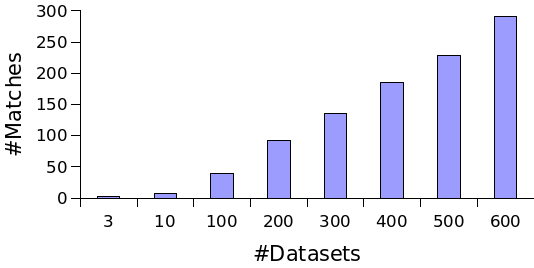
\includegraphics[width=0.5\textwidth]{img/LaundromatDsMatch.png}
        }%
        \subfigure[Time Dataset Matching]{%
           \label{fig:time600Laundromat}
           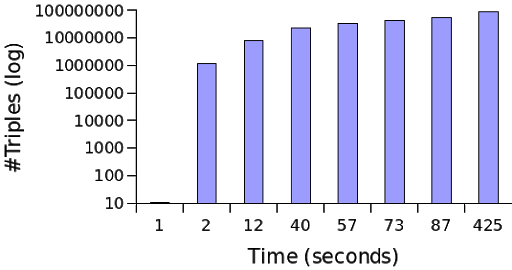
\includegraphics[width=0.5\textwidth]{img/time.png}
        }
%
    \end{center}
   \label{fig:subfigures}
   \caption{Dataset matching.}
\end{figure}

The time consumed can be observed on figure \ref{fig:time600Laundromat}, with 600 datasets from LODLaundromat\cite{beek2014lod}, which shows that 100 million triples were processed in less than 8 minutes, in which is a acceptable time, in which the starts to be time-consuming only after 1 million triples.

As we are using WimuQ\cite{ValdestilhasKcap} to identify datasets for a given SPARQL query together with our matching algorithm, we can answer the question (2) based on famous Sparql queries from two real-data federated SPARQL querying benchmarks \emph{LargeRDFBench} \cite{largerdfbench2017},\emph{FedBench} \cite{fedbench2011} and one non-federated real data SPARQL benchmark selected from \emph{FEASIBLE} \cite{feasible2015}. Thus, from the selected datasets we use our approach to select the datasets according to the properties and classes they share among them\footnote{In this case, all datasets identified by wimuQ are sharing properties and classes, that is why we are using the graph from \cite{ValdestilhasKcap}.}.
% \begin{figure}[htb]
% \centering
%     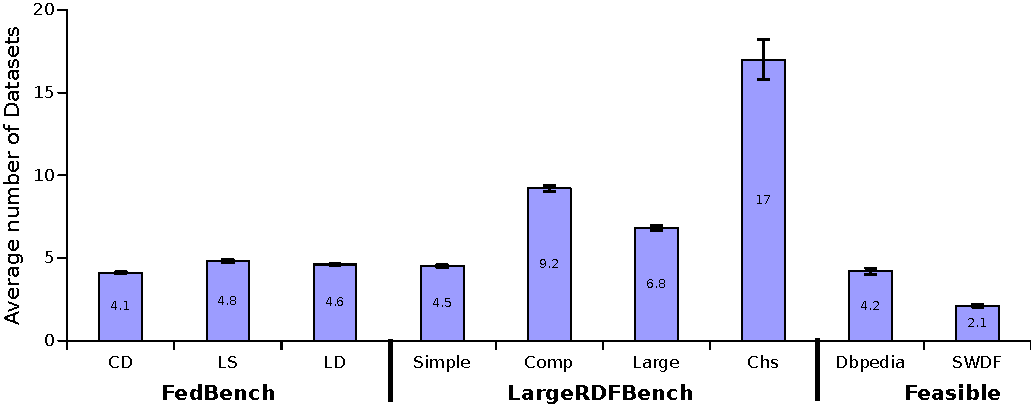
\includegraphics[width=\linewidth]{img/numberDatasets1.pdf}
% 	\caption{Average number of datasets discovered and queried by WimuQ\cite{ValdestilhasKcap} across different queries categories of the selected benchmarks.}
% 	\label{fig:numberDatasets1}
% \end{figure}

% To answer the question (3) we have the figure \ref{fig:md5Namespace} in which we can observe that all datasets from LODLaundromat are named with a MD5 code in which thanks to our approach you can know the domain and namespace information. There are \textbf{X} datasets from LODStats and \textbf{Y} SPARQL endpoints. \todo[inline]{Edgard, please verify and if not created yet, please create a graph/plot/chart fig:md5Namespace containing the info.}

To answer the question (3) we evaluate the dataset duplicated detection algorithm and the detection of dataset chunks.
From a 5446 datasets\footnote{A subset from those 600 datasets chosen previously} our algorithm detected 2272 duplicates and 1470 chunks in 3 hours.

The figure \ref{fig:identDuplicates} shows a case with 900 datasets chosen randomly, where we identified in 10 cases in which we can see the difference 

The figure \ref{fig:identChunks} show how many chunks we were able to identify among our sample data, in which lead us to know how segregated is data analysed, giving also the chance to know the complete dataset after the union of all chunks.

The current version of the index prototype has information about 539 SPARQL endpoints from LOD cloud\footnote{The list of is available here: \url{https://github.com/firmao/wimuT/blob/master/Endpoints_numtriples_lodcloud.csv}} and 915 HDT files from LOD Laundromat. We perform more than \num{1800000} comparisons in 88 hours.

Where \textbf{DsPropMatch} on the table \ref{tab:match} refers to the number of properties/classes the datasets share among each other.

\begin{table}[htb]
    \centering
    \begin{tabular}{ccccc} \hline
    \textbf{\#Datasets} & \textbf{\#DsropMatch} & \textbf{time (seconds)} & \textbf{\#triples} & \textbf{Synthetic} \\ \hline
    3 & 2 & 1 & 11 & Yes \\
    10 & 7 & 2 & 1198508 & no \\
    100 & 39 & 12 & 7996408 & no \\
    200 & 92 & 40 & 22982984 & no \\
    300 & 135 & 57 & 34792121 & no \\
    400 & 186 & 73 & 43864522 & no \\
    500 & 229 & 87 & 54227780 & no \\
    600 & 291 & 425 & 85041239 & no \\ \hline
    \end{tabular}
    \caption{Evaluation on the Match algorithm, where \textbf{DsPropMatch} refers to the number of properties/classes the datasets share among each other.}
    \label{tab:match}
\end{table}

We can observe the quantity of properties/classes that the datasets share related to the number of triples analysed. For instance, from 600 datasets, 291 matches where found, in which the number of triples was almost the double size of the previous case. Thus, the number of matches in this case cannot be directly related to the number of triples. Due to this fact, the quality of the datasets should be considerate a important phase.

We evaluate the accuracy of our matching algorithm with a small sample, where we can see at figure \ref{fig:fmeasure}, \ref{tab:TableFmeasure} and \ref{fig:runtimeSimilarMatch} the F-Measure and run-time on six famous pairs of datasets from\cite{georgala2018dynamic}, with those datasets we create a gold standard to compare, in which $P_1...P_n$ represents the pair of datasets and P1, P2 are datasets synthetically generated by the author, i.e. P3 represents the comparison between the datasets Abt and Buy.

\begin{figure}[H]
     \begin{center}
%
         \subfigure[Duplicates identified in 900 datasets. Y axis represents the number of datasets]{%
            \label{fig:identDuplicates}
            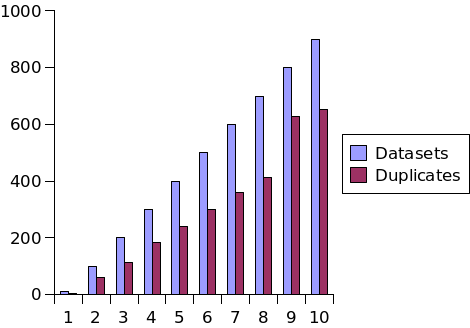
\includegraphics[width=0.5\textwidth]{img/DsDuplicate.png}
        }%
        \subfigure[Chunks identified in 900 datasets. Y axis represents the number of datasets]{%
           \label{fig:identChunks}
           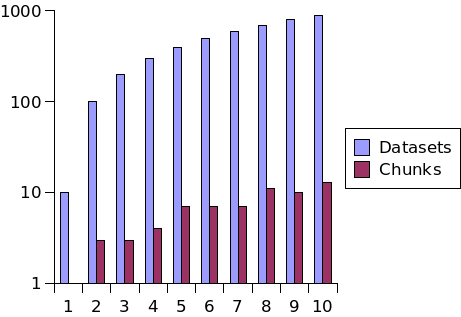
\includegraphics[width=0.5\textwidth]{img/DsChunks.png}
        }\\ %  ------- End of the first row ----------------------%
        \subfigure[F-measure on string similarity]{%
            \label{fig:fmeasure}
            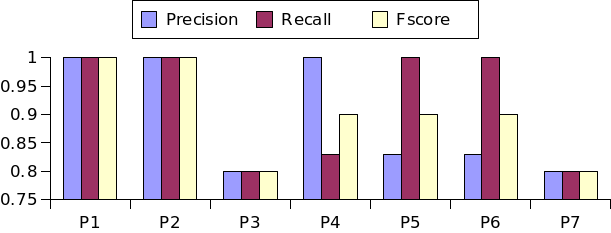
\includegraphics[width=0.5\textwidth]{img/fmeasure.png}
        }%
        \subfigure[Runtime on string similarity]{%
           \label{fig:runtimeSimilarMatch}
           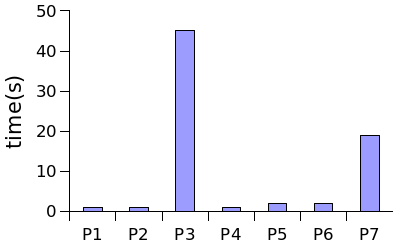
\includegraphics[width=0.5\textwidth]{img/runtime.png}
        }\\ %  ------- End of the first row ----------------------%
        \subfigure[Number of datasets identified by wimuQ using ReLOD]{%
            \label{fig:wimuQRelodDatasets}
            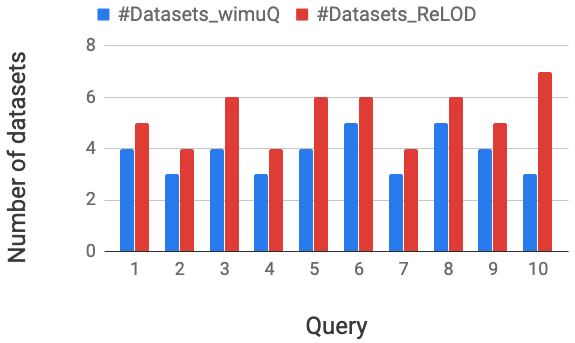
\includegraphics[width=0.5\textwidth]{img/wimuQRelodDatasets.png}
        }%
        \subfigure[Number of results identified by wimuQ using ReLOD. (Vertical axis in log scale)]{%
            \label{fig:wimuQRelodResults}
            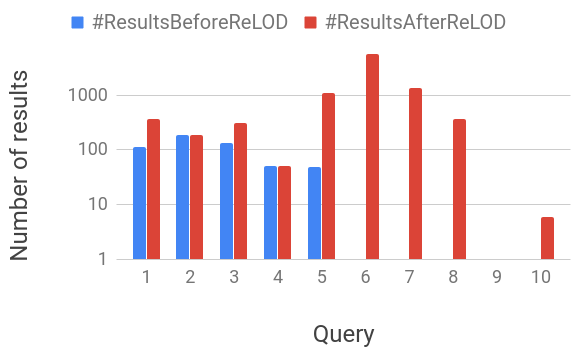
\includegraphics[width=0.5\textwidth]{img/wimuq_relod_results.png}
        }%
%
    \end{center}
    \caption{%
       Improvements of ReLOD.
     }%
   \label{fig:subfigures}
\end{figure}

The figure \ref{fig:dumps} shows that the majority of files from LODStats are in RDF/XML format.
Moreover, the endpoints are represented in greater numbers (78.6\%), the dominant file format is RDF with 84.1\% of the cases, and 56.2\% of errors occurred because Apache Jena was not able to perform SPARQL queries.
Among the HDT files from LOD Laundromat, 2.3\% of them could not be processed due to parsing errors.
Another relevant point is that 99.2\% of the URIs indexed with WIMU come from LOD Laundromat, due to 69.8\% of datasets from LODstats contain parser errors in which WIMU was not able to process the data.
%https://docs.google.com/spreadsheets/d/15kh8E4WllXG5Xdp1aL-JiHvnXAiVC6a8XqVUJ1gtMZ8/edit?usp=sharing

To answer the question (4) we selected 10 queries\footnote{The queries are available here: \url{https://github.com/firmao/LDatasetGenerator/blob/master/10_Queries_fedbench.txt}} from FedBench\cite{fedbench2011}, where we can observe on the figure \ref{fig:wimuQRelodDatasets} that thanks to the ReLOD approach we could increase the number of datasets identified by wimuQ, i.e., in query 5, using ReLOD allowed us to find 2 more datasets containing complementary information. 

On the other hand, the figure \ref{fig:wimuQRelodResults} reinforces that more datasets do not always imply in more results, i.e., in query 2 and 4, more datasets were identified, but the number of results did not change, in this case, the reason was that the datasets identified by ReLOD were practically the same with different property and class names. The results from queries 6 to 10 were only found thanks to the ReLOD approach\footnote{The query number 9 obtained only one result with the new approach.}.
